\documentclass{amsbook}
\usepackage{../Ceyhun}
\usepackage{../amsTurkish}

\begin{document}
    %%\hPage{ceyhun-154}
    \subsection{\underline{t-Kesitleme matrisinin gerçekleştirimi \hspace{3.4 in}}\\}

%%-----------------------------%%    
    \hspace{2cm}$ H(3)_{1} =
    \begin{array}{cc}
        & \begin{array}{c}
            1
        \end{array} \\
        \begin{array}{c}
            1
        \end{array} &
        \left[ \begin{array}{cc}
            1
        \end{array} \right]
    \end{array}$
    
%%-------------------------------%%%    
    \\ ya da
    
   \hspace{2cm}$ H(3)_{1} =
    \begin{array}{ccc}
        & \begin{array}{ccc}
            1& 2& 4 
        \end{array} \\
        \begin{array}{c}
            1 \\ 2 \\ 4
        \end{array} &
        \left[ \begin{array}{ccc}
            1 & 0 &  0 \\
            0 & 1 &  0 \\
            0 & 0 &  1 
        \end{array} \right]
    \end{array}$
\\
%%--------------------%%

de seçilebilirdi. Konuda daha çok ilerlemeden, doğru seçimin nasıl yapılacağını değgin herhangi birşey söyleyemeyiz.

%%---------------%%

$Ç_2$ ya da $Ç_1$ altçizgesindeki bütün düğümlerin büzüştürülüp, oluşabilecek tekçevrelerin de çizgeden atıldığını düşünürsek, elimizde Şekil \ref{fig:my_label}a da gösterilen çizgelerden biri kalacaktır.
%%-------------------%%
\begin{figure}[h]
    \centering
    \includegraphics{images/ceyhun-154-fig01.png}
    \label{fig:my_label}
\end{figure}

\end{document}